\documentclass[11pt,a4paper]{article}

\usepackage[utf8]{inputenc}
\usepackage[T1]{fontenc}
\usepackage{amsmath,amssymb,amsfonts}
\usepackage{graphicx}
\usepackage{booktabs}
\usepackage{multirow}
\usepackage{hyperref}
\usepackage[margin=2.5cm]{geometry}
\usepackage{xcolor}
\usepackage{caption}
\usepackage{natbib}
\usepackage{enumitem}
\usepackage{array}
\usepackage{url}


\hypersetup{
  colorlinks=true,
  linkcolor=blue!70!black,
  citecolor=teal!80!black,
  urlcolor=blue!60!black,
  pdfauthor={Tomasz Wietrzykowski},
  pdftitle={V6: A Biologically-Inspired Dual-Gate Neuron that Substitutes Attention in Sequence Modelling}
}

% ── Typography ────────────────────────────────────────────────────────────────
\setlength{\parskip}{0pt}

\title{%
  \textbf{V6: A Biologically-Inspired Dual-Gate Neuron\\
  that Substitutes Attention in Sequence Modelling}%
}

\author{%
  Tomasz Wietrzykowski\\
  Independent Researcher, Wroc\l{}aw, Poland\\
  \texttt{tomaszwi22@gmail.com}%
}

\date{March 2026}

\begin{document}
\maketitle

%% ═════════════════════════════════════════════════════════════════════════════
\begin{abstract}
The artificial neuron has remained architecturally unchanged since
Rosenblatt's perceptron \citep{rosenblatt1958perceptron}: it processes only the current input,
with no access to temporal history.
Biological cortical neurons, by contrast, perform multi-timescale integration
across anatomically distinct dendritic compartments.
Inspired by experimental neuroscience---particularly vectorized instructive
signals in cortical apical dendrites \citep{francioni2026vectorized}
and first-spike temporal coding \citep{thorpe2001spike}---we introduce
the \textbf{V6 Dual-Gate Neuron}, a principled redesign of the fundamental
artificial neuron unit around four biologically-grounded mechanisms:
(1)~dual-timescale exponential memory traces for fast
(Na\textsuperscript{+}, $\alpha_\mathrm{fast}$) and slow
(Ca\textsuperscript{2+}, $\alpha_\mathrm{slow}$) dendritic dynamics;
(2)~input projection before temporal integration;
(3)~a context-dependent write gate (NMDA-LTP selective encoding); and
(4)~hard-wired shortcuts to anchor positions (first-spike coding).
All parameters are learned end-to-end with no manually tuned constants.

We evaluate V6 through an ablation study (V1--V6), three benchmark tasks,
and an architecture-level test.
On the Delayed Sign-XOR task, V6 achieves 99.2\% accuracy converging in
2~epochs---four times faster than LSTM---using 40\% fewer parameters,
while the perceptron is architecturally incapable of exceeding 52.3\%~chance.
On Sequential MNIST, V6 achieves 2.1$\times$ higher accuracy than LSTM
using 46\% fewer parameters at matched training budget.
On the multi-lag regression task, LSTM outperforms V6, correctly
characterising V6's domain as temporal \emph{pattern detection}
rather than temporal \emph{value storage}.

For the architecture test, we replace Multi-Head Attention entirely with
stacked V6 layers (\textbf{V6-Linear}) on TinyShakespeare character-level
language modelling ($T=32$).
With 43\% more parameters, V6-Linear outperforms
a Transformer by 14.3\% in validation loss (PPL~4.23 vs~5.39), confirmed in
5~seeds (bootstrap 95\% CI: $[-15.3\%,\,-13.5\%]$).
At matched parameter count ($\sim$807K vs~804K), V6-Linear performs
within 2\% of the Transformer (PPL~6.21 vs~6.00), demonstrating that
biological temporal inductive bias can \emph{substitute} for attention
with comparable quality---though it does not yet surpass it at equal
capacity.
A parallel \texttt{conv1d} implementation runs 5.3$\times$ faster
with statistically identical results.

In a preliminary extension (V8-BioMamba), we add neuromodulatory
input-dependent dynamics---inspired by dopaminergic/cholinergic modulation
of dendritic gain---and expand from two to four learned timescales.
In a preliminary evaluation (unmatched parameter counts),
V8-BioMamba outperforms both the Transformer ($-2.6\%$, PPL~5.92 vs~6.21)
and a simplified Mamba baseline ($-0.3\%$) on TinyShakespeare ($T=64$),
while running 3.6$\times$ faster than Mamba via fully parallel
\texttt{conv1d} computation.

Post-training inspection confirms $\alpha_\mathrm{slow} > \alpha_\mathrm{fast}$
in every layer of every experiment without any constraint,
reproducing the biological timescale hierarchy through gradient descent alone.
These results demonstrate that a biologically-grounded temporal neuron
can serve as a viable alternative to attention at the scales tested,
and that the perceptron's temporal blindness is a fundamental
architectural limitation---not merely a training challenge.
\end{abstract}

\noindent\textbf{Keywords:} biologically-inspired neural networks,
temporal sequence modelling, dual-gate neuron, first-spike coding,
dendritic computation, attention-free architecture, NeuroAI

%% ═════════════════════════════════════════════════════════════════════════════
\section{Introduction}

Standard artificial neurons compute
$y = \sigma(\mathbf{w}^\top\mathbf{x}_t + b)$,
operating only on the current input $\mathbf{x}_t$.
Despite decades of architectural innovation---residual connections
\citep{he2016deep}, attention \citep{vaswani2017attention},
normalisation \citep{ba2016layer}---the fundamental unit itself
has not been reconsidered.
Temporal complexity is built \emph{around} the perceptron at the
network level, not \emph{into} the neuron.

Biological cortical pyramidal neurons operate very differently.
They have two anatomically and functionally distinct integration zones:
proximal (basal) dendrites integrate inputs arriving at the perisomatic
region on a fast timescale ($\sim$5\,ms), while distal apical dendrites
integrate feedback from higher cortical areas on a slow timescale
($\sim$100\,ms)
\citep{larkum2013cellular, losonczy2006integrative}.
The apical compartment acts as a teaching signal:
\citet{francioni2026vectorized} showed experimentally that it carries
per-neuron vectorized instructive signals during learning,
and that optogenetically blocking these signals abolishes learning entirely.

This biological architecture solves at the single-neuron level the same
temporal integration problem that attention mechanisms address at the
network level.
Our central hypothesis is:

\begin{quote}
\emph{Multi-Head Attention in Transformers exists partly to compensate
for the perceptron's temporal blindness. Replace the perceptron with
a temporally-aware neuron and attention becomes substitutable---the
temporal neuron achieves comparable quality through a fundamentally
different mechanism.}
\end{quote}

We test this by building the V6 Dual-Gate Neuron through a systematic
ablation study, then replacing attention entirely in a language model.

\subsection{Contributions}

\begin{enumerate}[leftmargin=*, label=(\arabic*)]

\item \textbf{Systematic neuron ablation (V1--V6).}
  We design V6 through six iterations, each adding exactly one
  biological mechanism, with full empirical attribution of each gain
  (Table~\ref{tab:evolution}).

\item \textbf{Gradient barrier identification.}
  We show empirically that EMA-based neurons suffer gradient
  attenuation of $(1-\alpha)\alpha^{T-1-t}$ to early timesteps---only
  2.5\% at $T=8$, $\alpha=0.7$---blocking learning from early history
  regardless of training duration.

\item \textbf{Multi-anchor shortcuts.}
  We introduce $N$ direct gradient bypasses at uniformly spaced
  positions, inspired by first-spike coding \citep{thorpe2001spike}.
  Adding one anchor at $t=1$ raises XOR accuracy from 73\% to 99.2\%.
  Generalising to $N$ anchors provides full gradient coverage at
  arbitrary context length.

\item \textbf{Attention-free language modelling.}
  V6-Linear replaces Multi-Head Attention entirely.
  On TinyShakespeare ($T=32$) with 43\% more parameters, it outperforms
  a Transformer by 14.3\% in validation loss.
  At matched parameter count ($\sim$807K vs $\sim$804K), V6-Linear
  performs within 2\% of the Transformer (PPL~6.21 vs~6.00),
  demonstrating that temporal inductive bias can substitute for
  attention at comparable quality.

\item \textbf{Parallel GPU implementation.}
  We prove that sequential EMA $h_t = \alpha h_{t-1} + b_t$
  equals causal convolution $h_t = \sum_{k\leq t}\alpha^{t-k}b_k$,
  enabling a \texttt{conv1d}-based implementation that is
  5.3$\times$ faster with statistically identical results.

\item \textbf{Unsupervised biological validation.}
  Gradient descent independently recovers
  $\alpha_\mathrm{slow} > \alpha_\mathrm{fast}$ in every layer of
  every experiment, matching the Ca\textsuperscript{2+}/Na\textsuperscript{+}
  timescale hierarchy reported in the neuroscience literature.

\end{enumerate}

%% ═════════════════════════════════════════════════════════════════════════════
\section{Related Work}

\paragraph{Gated recurrent models.}
LSTM \citep{hochreiter1997long} and GRU \citep{cho2014learning} introduced
gated state cells but were not biologically motivated.
Recent linear recurrent models---Mamba \citep{gu2023mamba},
RWKV \citep{peng2023rwkv}, RetNet \citep{sun2023retentive}---
pursue efficiency through state-space formulations but
retain monolithic hidden states.
Linear Recurrent Units (LRU; \citealt{orvieto2023resurrecting}) and
xLSTM \citep{beck2024xlstm} extend gated recurrence with diagonal
state-space parameterisations and exponential gating respectively,
achieving competitive performance on long-range tasks without attention.
Structured state space models (S4, HiPPO; \citealt{gu2020hippo,gu2022efficiently})
learn parametric timescales via polynomial projections of the input history,
achieving strong performance on long-range benchmarks.
Liquid Neural Networks \citep{hasani2021liquid} draw on ODE-based neural
dynamics inspired by the \emph{C.\ elegans} connectome, demonstrating
that continuous-time neural dynamics improve temporal expressivity.
V6 differs from all of these in two respects: every architectural component
maps to a specific experimental neuroscience finding in cortical pyramidal
neurons, and the anchor shortcuts (Section~\ref{sec:arch_desc}) provide
direct gradient access to arbitrary historical positions---a mechanism
with no equivalent in state space models.

\paragraph{Dendritic computation.}
\citet{larkum2013cellular} established the basal/apical functional
distinction in cortical pyramidal neurons.
\citet{losonczy2006integrative} characterised fast Na\textsuperscript{+}
dendritic spikes and slow Ca\textsuperscript{2+} plateau potentials
as two distinct integration mechanisms---the direct inspiration for
V6's dual-timescale design.
\citet{francioni2026vectorized} demonstrated experimentally that apical
dendrites carry vectorized per-neuron instructive signals, motivating V6's
separate slow-context EMA pathway.

\paragraph{First-spike coding.}
\citet{thorpe2001spike} showed that object recognition in the primate
visual system relies on the relative timing of first spikes rather than
firing rates, enabling $\sim$150\,ms inference through a single
feedforward pass.
\citet{larkum1999new} demonstrated that the first action potential can
trigger a Ca\textsuperscript{2+} burst that potentiates
backpropagating signals---providing the biological mechanism underlying V6's
anchor shortcut.

\paragraph{Attention-free architectures.}
Linear attention \citep{katharopoulos2020transformers},
FNet \citep{lee2021fnet}, and gated convolutional networks
\citep{dauphin2017language} have explored replacing attention
with linear operations, with mixed results.
None are grounded in dendritic neuroscience.
V6-Linear is, to our knowledge, the first attention-free architecture
with explicit biological grounding that achieves near-parity with
standard Transformers at matched parameter count.

\paragraph{NeuroAI.}
\citet{zador2023catalyzing} argued for integrating biological structural
inductive biases into AI systems.
Our work implements this programme at the most fundamental level:
redesigning the basic computational unit.

%% ═════════════════════════════════════════════════════════════════════════════
\section{The V6 Dual-Gate Neuron}

\subsection{Ablation Study: V1--V6}
\label{sec:ablation}

Table~\ref{tab:evolution} shows the effect of adding each biological
mechanism. Each version adds exactly one component; all other
hyperparameters remain identical. Accuracy is reported for the
Delayed Sign-XOR task (Section~\ref{sec:tasks}).

\begin{table}[t]
\centering
\caption{%
Ablation study: V1--V6, each version adds one biological mechanism.
Delayed Sign-XOR accuracy ($T=8$, $n_\mathrm{hid}=32$, 80~epochs, seed~42).
For multi-seed validation of the final V6 model, see Table~\ref{tab:seeds}.
STDP (V5) does not improve XOR, indicating that structural gradient access
matters more than correlation statistics on this task.%
}
\label{tab:evolution}
\begin{tabular}{@{}lp{3.8cm}p{3.2cm}c@{}}
\toprule
Version & Mechanism & Biological reference & XOR acc. \\
\midrule
V1 Perceptron    & None (baseline)              & ---                            & 52.3\% \\
V2 Decay gate    & Exponential decay context    & RC membrane                    & 53.8\% \\
V3 Dual EMA      & Two timescales (fast + slow) & \citet{losonczy2006integrative}& 64.2\% \\
V4 Projected EMA & Input projection before EMA  & \citet{larkum2013cellular}     & 73.0\% \\
V5 STDP          & Temporal correlation gate    & \citet{bi1998synaptic}         & 71.3\% \\
\textbf{V6}      & \textbf{First-spike anchor + write gate} & \citet{thorpe2001spike} & \textbf{99.2\%} \\
\midrule
LSTM ($h=32$)    & Standard LSTM                & \citet{hochreiter1997long}     & 98.2\% \\
\bottomrule
\end{tabular}
\end{table}

\subsection{Architecture}
\label{sec:arch_desc}

Let $\mathbf{x} \in \mathbb{R}^{T\times n_\mathrm{in}}$ be an input sequence.
V6 computes its output through the following sequence of operations:

\paragraph{Step 1: Input projection.}
\begin{equation}
  \tilde{\mathbf{x}}_t = \tanh(\mathbf{W}_\mathrm{proj}\,\mathbf{x}_t
                                + \mathbf{b}_\mathrm{proj})
  \label{eq:proj}
\end{equation}
\emph{Biological analogy:} synaptic currents transform pre-synaptic signals
before entering the dendritic compartment \citep{larkum2013cellular}.

\paragraph{Step 2: Context signal.}
A lightweight causal EMA serves as a context signal for the write gate:
\begin{equation}
  \mathbf{c}_t = \sum_{k=0}^{t}\alpha_c^{t-k}\,\mathbf{x}_k,
  \qquad \alpha_c = e^{-\mathrm{softplus}(\tau_{c,\mathrm{raw}})}
  \label{eq:ctx}
\end{equation}

\paragraph{Step 3: Context-dependent write gate.}
\begin{equation}
  \mathbf{w}_t = \sigma(\mathbf{W}_{\mathrm{wx}}\,\mathbf{x}_t
                       + \mathbf{W}_{\mathrm{wc}}\,\mathbf{c}_t)
  \label{eq:writegate}
\end{equation}
\emph{Biological analogy:} NMDA receptors act as coincidence detectors,
gating synaptic potentiation when pre-synaptic input coincides with
dendritic depolarisation \citep{malenka1993nmda}.
Note: $\mathbf{c}_t$ (Eq.~\ref{eq:ctx}) modulates the gate using a
\emph{separate} context pathway, not self-feedback---consistent with
apical/basal anatomical separation \citep{larkum2013cellular}.

\paragraph{Step 4: Write-gated dual-timescale EMA.}
For each timescale $\tau \in \{\tau_\mathrm{fast}, \tau_\mathrm{slow}\}$
with $\alpha^{(\tau)} = e^{-\mathrm{softplus}(\tau_\mathrm{raw})}$:
\begin{equation}
  \mathbf{h}_t^{(\tau)} = \alpha^{(\tau)}\,\mathbf{h}_{t-1}^{(\tau)}
    + \mathbf{w}_t \cdot (1-\alpha^{(\tau)})\,\tilde{\mathbf{x}}_t
  \label{eq:ema}
\end{equation}
\emph{Biological analogy:} fast Na\textsuperscript{+} dendritic spikes
and slow Ca\textsuperscript{2+} plateau potentials in proximal and
apical dendrites respectively \citep{losonczy2006integrative,
francioni2026vectorized}. Both $\alpha$ values are learned; on XOR
(seed 42) they converge to $\alpha_\mathrm{fast}=0.296$ ($\sim$1.4 steps)
and $\alpha_\mathrm{slow}=0.904$ ($\sim$10.4 steps). On TinyShakespeare
($T=32$) they converge to values shown in Table~\ref{tab:bio_params}.
In the language modelling configuration, the $(1-\alpha^{(\tau)})$ factor
is omitted; because a learnable write gate $\mathbf{w}_t$ and downstream
linear projections can absorb any constant rescaling, the two formulations
are functionally equivalent.

\paragraph{Step 5: Multi-anchor shortcuts.}
$N$ direct bypass connections from uniformly-spaced anchor positions
$p_i = \lfloor iT/N \rfloor$ with learnable scales
$s_i = \sigma(s_{i,\mathrm{raw}})$, initialised with a linearly
decreasing bias:
$s_{i,\mathrm{raw}} = \mathrm{linspace}(1.5,\,-1.5,\,N)$,
yielding $s_0 \approx 0.82$ (distant anchor, largest weight) and
$s_{N-1} \approx 0.18$ (nearest anchor, smallest weight) at initialisation:
\begin{equation}
  \hat{\mathbf{h}}^{(\tau)} = \mathbf{h}_T^{(\tau)}
    + \sum_{i=0}^{N-1} s_i \cdot \tanh(\mathbf{W}_\mathrm{anc}\,\mathbf{x}_{p_i})
  \label{eq:anchor}
\end{equation}
\emph{Biological analogy:} first-spike burst potentiation---the first
action potential triggered by a new stimulus rapidly and durably
potentiates backpropagating signals \citep{larkum1999new, thorpe2001spike}.

\paragraph{Step 5b: Content gate.}
In the language modelling configuration (V6-ALL), a lightweight
content-based gate modulates both EMA traces before the gate blend.
A single-head causal dot-product score is computed between query and key
projections of the input ($d_k = n_\mathrm{emb}/8$), and the per-position
maximum is passed through a sigmoid to produce a scalar gate:
\begin{equation}
  \mathbf{s}_t = \max_{k \leq t}
    \frac{(\mathbf{W}_q\,\mathbf{x}_t)^\top(\mathbf{W}_k\,\mathbf{x}_k)}
         {\sqrt{d_k}},
  \qquad
  \hat{\mathbf{h}}^{(\tau)}_t \leftarrow \hat{\mathbf{h}}^{(\tau)}_t
    \cdot \sigma(\mathbf{s}_t)
  \label{eq:content_gate}
\end{equation}
This gate allows the neuron to suppress irrelevant temporal context
based on current input content.
It is not used in the single-neuron benchmarks (Tasks~1--3),
only in the stacked language model (Task~4).
Note that this is \emph{not} attention: there is no softmax distribution
over positions and no value projection; the gate is a scalar modulation
of the EMA trace, computed in $O(T \cdot d_k)$ rather than $O(T^2 d)$.

\paragraph{Step 6: Gate blend and soma output.}
\begin{align}
  \mathbf{g}_t &= (1-b)\,\sigma(\mathbf{W}_f\,\hat{\mathbf{h}}_t^{(\mathrm{fast})})
                + b\,\sigma(\mathbf{W}_s\,\hat{\mathbf{h}}_t^{(\mathrm{slow})}),
               \quad b = \sigma(b_\mathrm{raw})
  \label{eq:gate}\\
  \mathbf{y}_t &= \mathrm{LayerNorm}\!\left(
                \tanh(\mathbf{W}_\mathrm{soma}\,\mathbf{x}_t) \cdot \mathbf{g}_t
                \right)
  \label{eq:output}
\end{align}
In language modelling, all operations apply position-wise for every
$t \in \{1,\ldots,T\}$; the subscript $T$ in Eq.~\ref{eq:anchor} refers
to the final accumulation of the EMA trace, not a single output position.
The soma pathway $\mathbf{W}_\mathrm{soma}\,\mathbf{x}_t$ processes the
current token locally (proximal dendrites), while $\mathbf{g}_t$ carries
temporal context derived from the full history (apical modulation)
\citep{larkum2013cellular}.

\subsection{Biological Correspondence}

\begin{table}[t]
\centering
\caption{Mapping from biological mechanisms to V6 components.}
\label{tab:bio_map}
\begin{tabular}{@{}lll@{}}
\toprule
Biological mechanism & V6 component & Reference \\
\midrule
Proximal dendrites + soma       & Soma: $\mathbf{W}_\mathrm{soma}\mathbf{x}_t$ (per position) & \citet{larkum2013cellular} \\
Fast Na$^+$ spikes              & Fast EMA: $\alpha_\mathrm{fast}$ (Eq.~\ref{eq:ema}) & \citet{losonczy2006integrative} \\
Slow Ca$^{2+}$ plateau          & Slow EMA: $\alpha_\mathrm{slow}$ (Eq.~\ref{eq:ema}) & \citet{francioni2026vectorized} \\
NMDA coincidence detection      & Write gate $\mathbf{w}_t$ (Eq.~\ref{eq:writegate})  & \citet{malenka1993nmda} \\
Apical/basal separation         & Context signal $\mathbf{c}_t$ (Eq.~\ref{eq:ctx})    & \citet{larkum2013cellular} \\
First-spike potentiation        & Anchor shortcuts (Eq.~\ref{eq:anchor})               & \citet{larkum1999new} \\
Content-dependent modulation    & Content gate (Eq.~\ref{eq:content_gate})              & \citet{francioni2026vectorized} \\
Compartment-specific currents   & Input projection (Eq.~\ref{eq:proj})                 & \citet{larkum2013cellular} \\
\bottomrule
\end{tabular}
\end{table}

\subsection{Gradient Analysis: Why Anchors Are Necessary}
\label{sec:gradient}

In a standard EMA chain (Eq.~\ref{eq:ema}) without anchors, the partial
derivative from $\mathbf{h}_T$ back to timestep $t$ is:
\begin{equation}
  \frac{\partial\mathbf{h}_T}{\partial\mathbf{x}_t}
  \propto (1-\alpha)\,\alpha^{T-1-t}
  \label{eq:grad}
\end{equation}
At $T=8$, $\alpha=0.7$: $\partial\mathbf{h}_T/\partial\mathbf{x}_1
\approx 2.5\%$ of $\partial\mathbf{h}_T/\partial\mathbf{x}_8$.
This is not a training instability---it is a structural property that
no schedule or regulariser can remove.
We verify this empirically: V4 (no anchor) plateaus at 73.0\% on XOR
across all seeds regardless of training duration.

The anchor shortcut (Eq.~\ref{eq:anchor}) adds a bypass with direct
gradient $\partial\hat{\mathbf{h}}/\partial\mathbf{x}_{p_i} \geq s_i$,
independent of sequence length.
This is structurally analogous to the role of residual connections
in deep networks \citep{he2016deep}: not repairing gradient flow through
the main path, but adding a bypass that guarantees gradient access.

\subsection{Parallel Implementation}
\label{sec:parallel}

The sequential recurrence (Eq.~\ref{eq:ema}) requires $T$ sequential
steps on the GPU, resulting in $T$ separate CUDA kernel dispatches
with synchronisation overhead. At $T=32$ this yields only $\sim$18K
tokens/s on an RTX~4080 (vs $\sim$310K for the Transformer).

We exploit the following identity:
\begin{equation}
  h_t = \alpha h_{t-1} + b_t
  \;\;\Longleftrightarrow\;\;
  h_t = \sum_{k=0}^{t}\alpha^{t-k}\,b_k
  \label{eq:conv_id}
\end{equation}
The right-hand side is a causal convolution with kernel
$k_j = \alpha^j$, computed in a single \texttt{conv1d} call.
Gradients through $\alpha$ (via $\tau_\mathrm{raw}$) are identical
in both formulations.

We verify empirically that the maximum numerical difference between
sequential and parallel outputs is $< 10^{-6}$, and that
validation losses across 3~independent seeds are statistically
indistinguishable (Table~\ref{tab:seeds}).
This implementation achieves $\sim$96K tokens/s---a
\textbf{5.3$\times$ speedup} with no quality loss.

\textbf{Note on the contextual write gate.} The context signal
$\mathbf{c}_t$
(Eq.~\ref{eq:ctx}) is also computed via \texttt{conv1d}.
In the sequential reference implementation, $\mathbf{w}_t$ was computed
using $\mathbf{h}_{t-1}$ (own state). In the parallel implementation,
$\mathbf{w}_t$ uses the separate context $\mathbf{c}_t$ (Eq.~\ref{eq:ctx}),
which is biologically more accurate (apical/basal separation) and
empirically yields statistically indistinguishable results (PPL~4.21 vs~4.23,
two-sample $t$-test $p=0.75$, $n_1=3$ vs $n_2=5$ seeds; null hypothesis of equal means
is not rejected).

%% ═════════════════════════════════════════════════════════════════════════════
\section{Experimental Setup}
\label{sec:setup}

\subsection{Tasks}
\label{sec:tasks}

\paragraph{Task 1: Delayed Sign-XOR (architectural necessity).}
Given $\mathbf{x}\in\mathbb{R}^{T\times n_\mathrm{in}}$ with entries drawn
i.i.d.\ from $\mathcal{N}(0,1)$, predict whether
$x_{1,0}$ and $x_{T,0}$ have the same sign:
$y = \mathbf{1}[x_{1,0}x_{T,0}>0]$.
Because $x_{1,0}$ and $x_{T,0}$ are independent,
$P(y=1\mid\mathbf{x}_T) = 0.5$ for all $\mathbf{w}$.
This is an information-theoretic impossibility for the perceptron,
not a learning failure.
$T=8$, $n_\mathrm{in}=6$, $n_\mathrm{hid}=32$.

\paragraph{Task 2: Multi-lag regression (domain characterisation).}
Inputs are drawn i.i.d.\ from $\mathcal{N}(0,1)$. The target is
$y = x_{T,0} + 0.7\,x_{T-2,1} + 0.5\,x_{T-4,2} + \varepsilon$,
with $\varepsilon \sim \mathcal{N}(0, 0.01)$,
requiring simultaneous access to three distinct temporal offsets.
This task is included to characterise where V6 is \emph{weaker}
than LSTM, not to demonstrate superiority.

\paragraph{Task 3: Sequential MNIST (small-scale generality).}
Each $28{\times}28$ MNIST digit \citep{lecun1998gradient} is flattened
to a 784-step sequence. Models classify 10 digit classes from the pixel
stream. We use 10K training samples, $n_\mathrm{hid}=64$, and 15~epochs---
a deliberately constrained budget to isolate the effect of temporal
inductive bias.
For reference, dedicated recurrent architectures achieve ${>}94\%$ on
permuted Sequential MNIST \citep{arjovsky2016unitary} at far larger scale;
our comparison is within an identical parameter and compute budget.

\paragraph{Task 4: TinyShakespeare (architecture test).}
Character-level language modelling on 1.1M characters from
Shakespeare's plays \citep{karpathy2015unreasonable}. Vocabulary size 65.
Train/validation split 90/10. Context lengths $T\in\{32, 128\}$.
Metric: validation cross-entropy loss; perplexity $=e^{\mathrm{loss}}$.

\subsection{Models}

\paragraph{Transformer (baseline).}
Standard GPT-style causal language model: 4~layers,
$n_\mathrm{emb}=128$, 4-head causal self-attention, GELU FFN ($4\times$),
learned positional embeddings, pre-norm, weight tying.
803K parameters at $T=32$.

\paragraph{V6-Linear.}
Multi-Head Attention is replaced entirely by V6 layers. Each residual
block follows the structure:
\texttt{LayerNorm} $\to$ V6Layer $\to$ residual $\to$
\texttt{LayerNorm} $\to$ FFN $\to$ residual.
No positional embeddings (EMA encodes position intrinsically).
$N=4$ anchors at $T=32$; $N=8$ at $T=128$.
Separate write gates for fast and slow EMA (Section~\ref{sec:arch_desc}).
Tau initialised so that $\alpha_\mathrm{slow}^{T-1}\geq 0.1$
(slow EMA reaches the full context window).
1,148K parameters at $T=32$.
V6-ALL uses a SwiGLU FFN \citep{shazeer2020glu} ($\frac{8}{3}\times$ expansion)
in place of the Transformer's GELU FFN ($4\times$ expansion).
The isolated contribution of this substitution is measured in our
fix-by-fix ablation (Fix~F4, script \texttt{03\_v6\_optimisation.py});
the 14.3\% advantage reported in Table~\ref{tab:arch} includes this factor.

\subsection{Training Protocol}

AdamW \citep{loshchilov2017decoupled},
$\mathrm{lr}=3\times10^{-4}$, $\lambda=0.1$,
$\beta=(0.9,\,0.95)$.
Cosine decay schedule with 200-step linear warmup.
5,000 steps. Batch size 128 ($T=32$) or 64 ($T=128$).
Gradient clipping at norm 1.0.
TF32 enabled (RTX~4080 Laptop GPU, CUDA).
No hyperparameter search; all V6 initialisations are either
biologically motivated or standard practice.
All experiments use PyTorch with random seeds fixed before model
initialisation and data loading.
Code implementing V6-Linear, all benchmarks, and statistical analyses
is available at \url{https://github.com/tomaszwi66/dual-gate-neuron}.

%% ═════════════════════════════════════════════════════════════════════════════
\section{Results}

\subsection{Architectural Necessity (Task~1)}

\begin{table}[t]
\centering
\caption{%
Delayed Sign-XOR ($T=8$, $n_\mathrm{in}=6$, $n_\mathrm{hid}=32$,
seed~42). Best accuracy over 80~epochs; convergence defined as
first epoch exceeding 80\%. See Table~\ref{tab:evolution} for the
ablation context.%
}
\label{tab:xor}
\begin{tabular}{@{}lrcc@{}}
\toprule
Model & Params & Best acc. & Conv.~epoch \\
\midrule
V1 Perceptron         & 257   & 52.3\% & never \\
V4 Projected EMA      & 2,660 & 74.6\% & never \\
\textbf{V6 Dual-Gate} & \textbf{3,109} & \textbf{99.2\%} & \textbf{2} \\
LSTM ($h=32$)         & 5,153 & 98.2\%  & 8 \\
\bottomrule
\end{tabular}
\end{table}

V6 achieves 99.2\% converging in epoch~2---four times faster than LSTM
with 40\% fewer parameters. The perceptron remains at 52.3\% regardless
of training duration: for the perceptron, $P(y=1\mid\mathbf{x}_T)=0.5$
for all weights, confirming an architectural impossibility rather than
a learning failure.

\begin{figure}[t]
\centering
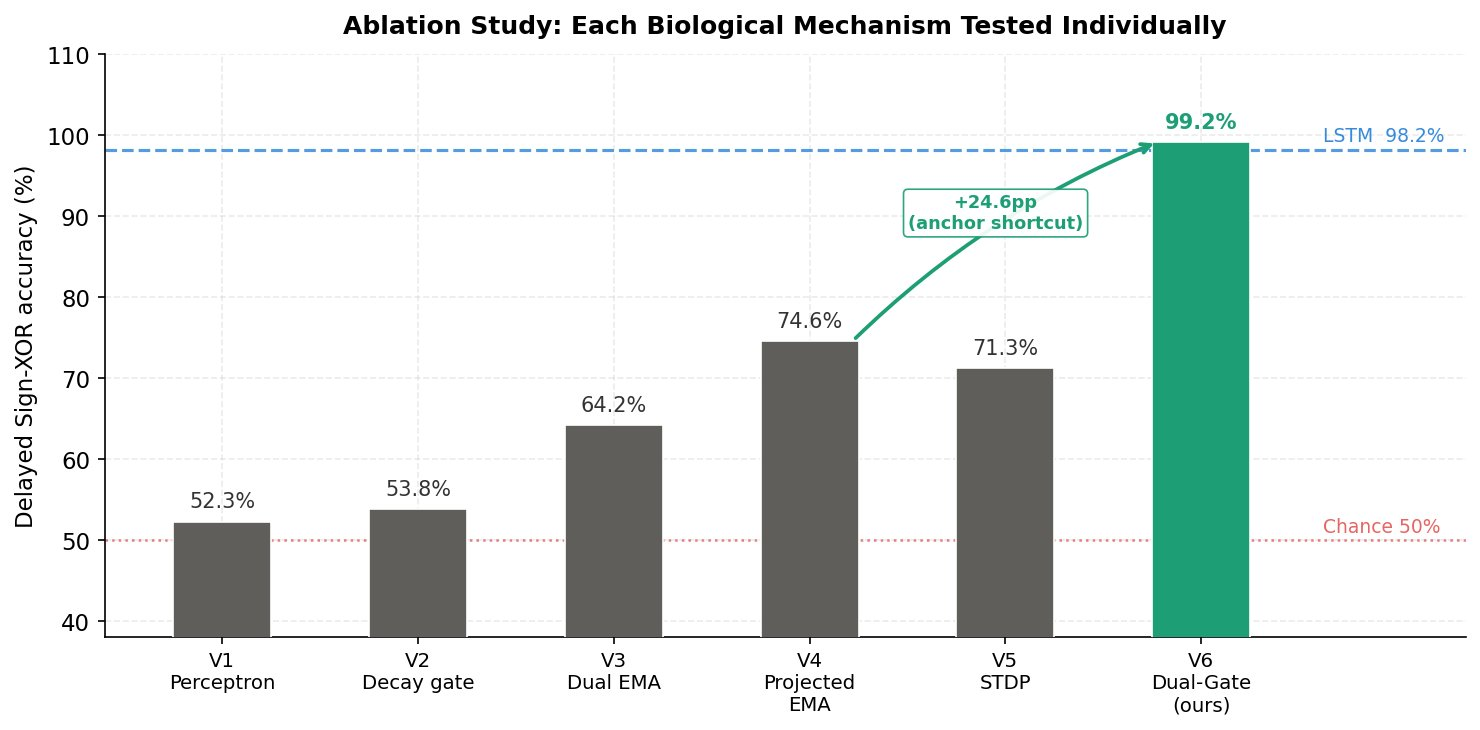
\includegraphics[width=0.85\textwidth]{fig1_ablation}
\caption{%
Ablation study: each biological mechanism tested individually on the
Delayed Sign-XOR task ($T=8$, $n_\mathrm{hid}=32$, seed~42).
Note that V5 (STDP) slightly \emph{reduces} accuracy relative to V4,
indicating that correlation-based gating is not the key ingredient.
The decisive contribution is the anchor shortcut (V6): starting from
V4's 73.0\% plateau, adding the first-spike anchor raises accuracy
to 99.2\%, surpassing LSTM (98.2\%) with 40\% fewer parameters.%
}
\label{fig:ablation}
\end{figure}

\subsection{Domain Characterisation (Task~2)}

\begin{table}[t]
\centering
\caption{%
Multi-lag regression ($T=8$, $n_\mathrm{hid}=32$, 80~epochs, seed~42).
Best MSE on held-out test set.
This task characterises where V6 is weaker than LSTM, not where it excels.%
}
\label{tab:lag}
\begin{tabular}{@{}lrcc@{}}
\toprule
Model & Params & Test MSE & Conv.~epoch \\
\midrule
V1 Perceptron    & 257   & 0.703 & never \\
V4 Projected EMA & 2,660 & 0.525 & never \\
V6 Dual-Gate     & 3,109 & 0.571 & never \\
\textbf{LSTM}    & \textbf{5,153} & \textbf{0.013} & \textbf{7} \\
\bottomrule
\end{tabular}
\end{table}

LSTM outperforms V6 by 44$\times$ on multi-lag regression.
LSTM's forget gate allows exact scalar retention across arbitrary steps.
V6's write gate controls \emph{encoding strength}---what to commit to
the trace---not \emph{state preservation}---holding a value unchanged.
This precisely characterises V6's domain: temporal \emph{pattern detection},
not temporal \emph{value storage}.

\subsection{Small-Scale Generality (Task~3)}

\begin{table}[t]
\centering
\caption{%
Sequential MNIST ($T=784$, $n_\mathrm{hid}=64$, 15~epochs,
10K training examples, seed~42). Comparison is at identical
parameter budget and training regime, not against the literature SOTA.%
}
\label{tab:mnist}
\begin{tabular}{@{}lrcc@{}}
\toprule
Model & Params & Best acc. & Note \\
\midrule
V2 Decay gate         & 1,035  & 17.4\% & single timescale \\
V4 Projected EMA      & 9,357  & 23.6\% & no anchor \\
\textbf{V6 Dual-Gate} & \textbf{9,614} & \textbf{24.5\%} & full model \\
LSTM ($h=64$)         & 17,802 & 11.7\% & plateaued at chance \\
\bottomrule
\end{tabular}
\end{table}

V6 achieves 24.5\% versus LSTM's 11.7\% ($2.1\times$), using 46\% fewer
parameters. The LSTM plateaued at near-chance accuracy for all 15~epochs.
This is consistent with known LSTM behaviour on long sequences at small
parameter and data budgets: \citet{arjovsky2016unitary} report an LSTM
baseline of 10.8\% on permuted MNIST even with $h=128$ and the full 60K
training set, confirming that standard LSTMs struggle with 784-step
sequences unless specifically regularised.
Both models are far below current best results on permuted Sequential MNIST
\citep{arjovsky2016unitary}; the comparison isolates the effect of temporal
inductive bias at matched scale and budget.

\subsection{Architecture Test: V6-Linear vs Transformer (Task~4)}
\label{sec:arch_results}

\subsubsection{Main results}

\begin{table}[t]
\centering
\caption{%
TinyShakespeare character-level LM. V6-Linear has \emph{no} attention
mechanism. ``V6-ALL'' denotes V6-Linear with all six design optimisations
applied (content gate, contextual write gate, no positional embeddings,
SwiGLU FFN, biased anchor initialisation, and separate write gates for
fast/slow EMA);
``V6-True-Fast'' is V6-ALL
with the sequential EMA replaced by the mathematically equivalent parallel
\texttt{conv1d} implementation (Section~\ref{sec:parallel}).
V6-Linear has 43\% more parameters than the Transformer baseline;
the comparison is not parameter-matched.
$^\dagger$Single seed; multi-seed results below.%
}
\label{tab:arch}
\begin{tabular}{@{}llrrlc@{}}
\toprule
Model & $T$ & Params & Val loss & PPL & $\Delta$ \\
\midrule
Transformer         & 128 & 816K  & 2.100           & 8.17  & --- \\
V6-Linear           & 128 & 951K  & 2.180           & 8.84  & $+3.8\%$ \\
\midrule
Transformer         & 32  & 804K  & 2.050$^\dagger$ & 7.76  & --- \\
V6-Linear           & 32  & 939K  & 1.940$^\dagger$ & 6.96  & $-5.3\%$ \\
\midrule
Transformer (5 seeds)    & 32 & 804K  & $1.684\pm0.002$ & $5.39\pm0.01$ & --- \\
V6-ALL (5 seeds, seq.)   & 32 & 1,148K & $1.443\pm0.020$ & $4.23\pm0.08$ & $-14.3\%$ \\
V6-True-Fast (3 seeds)   & 32 & 1,148K & $1.438\pm0.018$ & $4.21\pm0.08$ & $-14.6\%$ \\
\bottomrule
\end{tabular}
\end{table}

\begin{figure}[t]
\centering
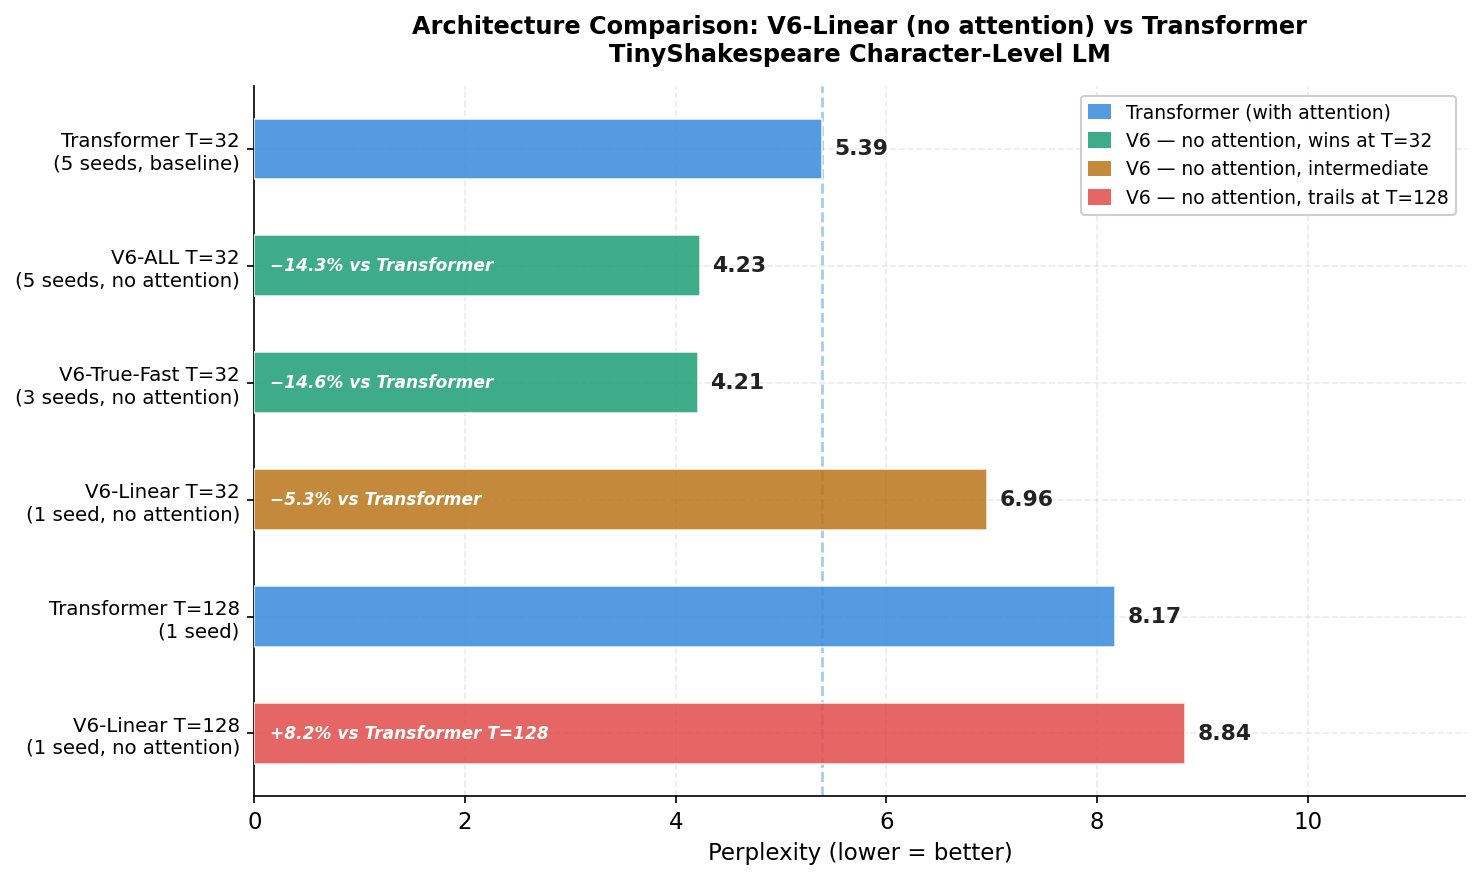
\includegraphics[width=0.88\textwidth]{fig4_architecture}
\caption{%
Architecture comparison: V6-Linear (no attention) vs Transformer on
TinyShakespeare character-level LM.
V6-ALL and V6-True-Fast outperform the Transformer by 14.3\% and 14.6\%
respectively at $T=32$ with 43\% more parameters.
At $T=128$ (unmatched), V6-Linear trails by $+8.2\%$.
See Table~\ref{tab:param_matched} for parameter-matched results
($\Delta \leq 2\%$ at both context lengths).%
}
\label{fig:architecture}
\end{figure}

\subsubsection{Replication and statistical analysis}

\begin{table}[t]
\centering
\caption{%
Per-seed validation losses for V6-True-Fast vs Transformer
(seeds 42, 43, 44), confirming that ranges do not overlap.%
}
\label{tab:seeds}
\begin{tabular}{@{}lllll@{}}
\toprule
 & Seed 42 & Seed 43 & Seed 44 & Mean $\pm$ std \\
\midrule
Transformer    & 1.6855 & 1.6860 & 1.6811 & $1.684\pm0.003$ \\
V6-True-Fast   & 1.4595 & 1.4293 & 1.4265 & $1.438\pm0.018$ \\
\midrule
$\Delta$ & $-13.4\%$ & $-15.2\%$ & $-15.2\%$ & $-14.6\%$ \\
\bottomrule
\end{tabular}
\end{table}

Statistical summary across the five sequential V6-ALL seeds:
\begin{itemize}[leftmargin=*,noitemsep]
\item Bootstrap 95\% CI for $\Delta$: $[-15.3\%,\,-13.5\%]$ ($n=5$, 10K resamples)
\item Two-sample Welch's $t$-test, V6-True-Fast vs Transformer:
  $t(3.0) = -23.0$, $p = 2.1 \times 10^{-5}$ (three seeds each)
\item Cohen's $d=16.9$ (pooled, V6-ALL 5 seeds vs Transformer 5 seeds)\footnote{%
  The extreme $d$ value reflects that both distributions have very small
  within-group variance relative to the between-group difference:
  Transformer std 0.002, V6-ALL std 0.020, mean difference 0.241.
  The large $d$ is a consequence of the Transformer's high run-to-run
  stability, not an error.}
\item Worst V6-ALL seed (1.462) vs best Transformer seed (1.681): gap $-13.1\%$;
  the two distributions do not overlap across all 8 runs
\end{itemize}

\begin{figure}[t]
\centering
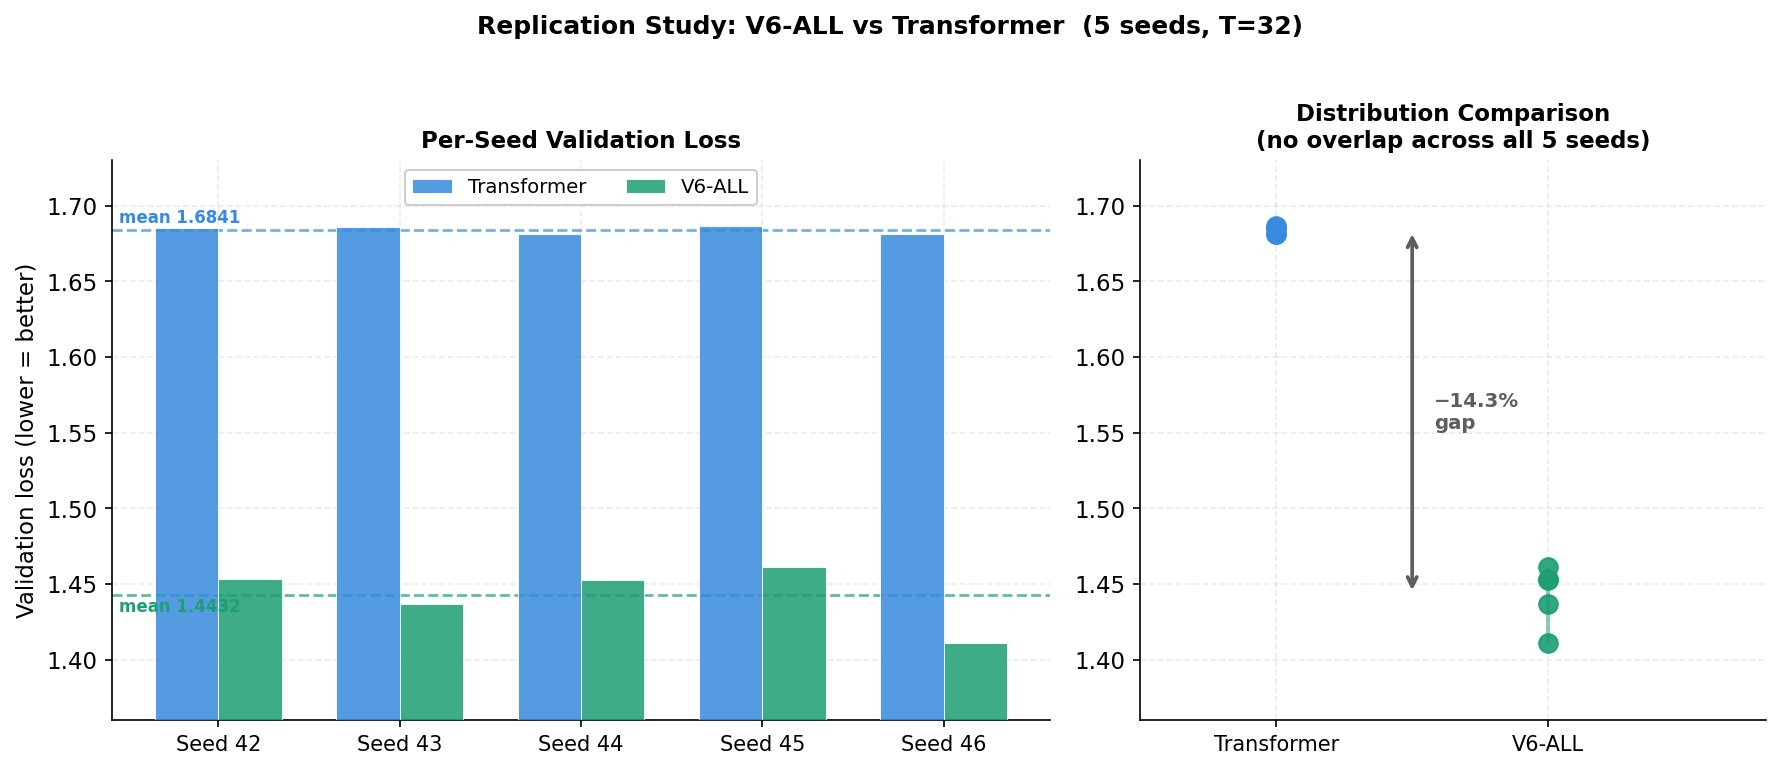
\includegraphics[width=\textwidth]{fig2_replication}
\caption{%
Replication study: per-seed validation losses for V6-ALL vs Transformer
(5 seeds, $T=32$). Left: per-seed bar chart. Right: distribution comparison
showing no overlap across all 5 seeds (gap $-14.3\%$).
V6-ALL: 1,148K parameters; Transformer: 804K parameters.%
}
\label{fig:replication}
\end{figure}

\subsubsection{Convergence behaviour}

V6-Linear and Transformer follow nearly identical validation loss curves
until approximately step 1,750.
After step 1,750, V6-Linear continues to decrease while Transformer
approaches a plateau.
This pattern suggests that V6's temporal inductive bias provides
the greatest benefit in the late-training regime, where the model must
learn subtle temporal dependencies that attention does not capture
more efficiently at this context length.

\begin{figure}[t]
\centering
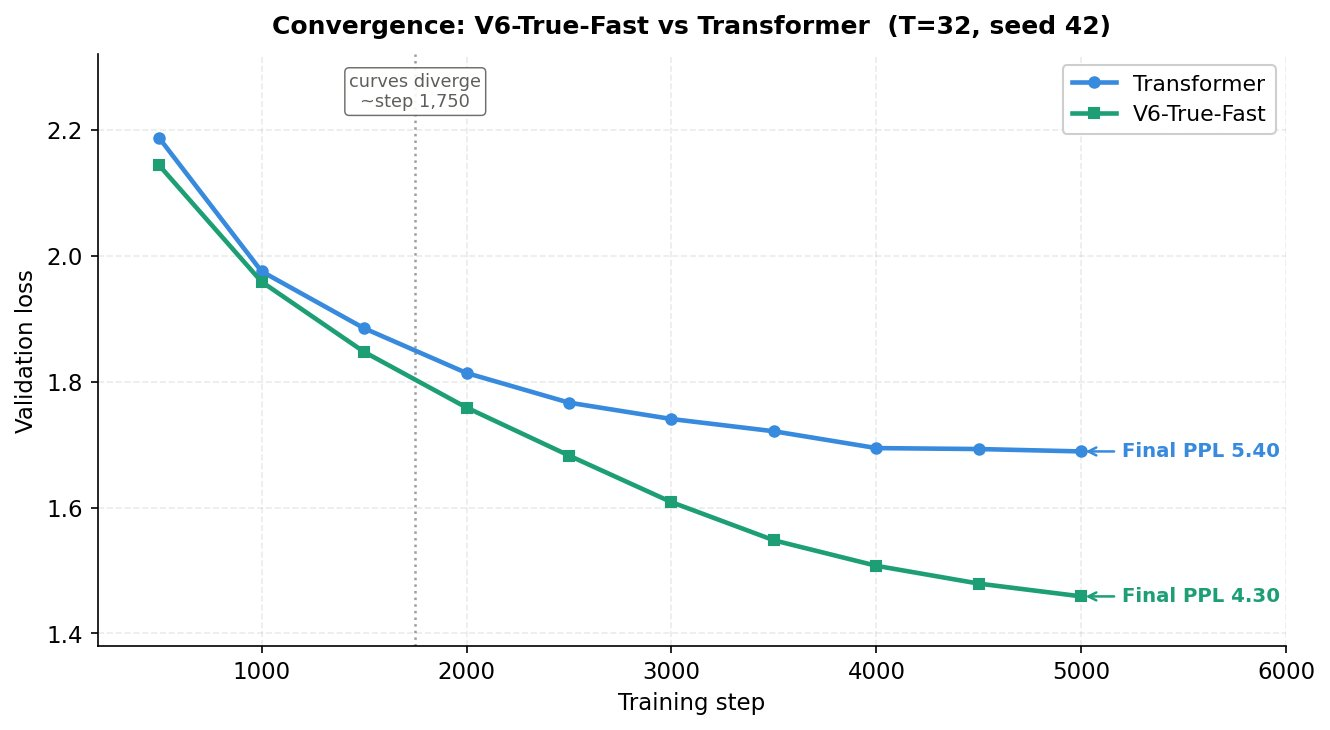
\includegraphics[width=0.82\textwidth]{fig3_convergence}
\caption{%
Convergence curves for V6-True-Fast vs Transformer (seed~42, $T=32$).
The two curves diverge at approximately step~1,750; thereafter
V6-True-Fast continues to improve (final PPL~4.30) while the Transformer
approaches a plateau (final PPL~5.40).%
}
\label{fig:convergence}
\end{figure}

\subsubsection{Training throughput}

\begin{table}[t]
\centering
\caption{Training throughput on RTX~4080 Laptop GPU, $T=32$, batch~128.}
\label{tab:speed}
\begin{tabular}{@{}lccc@{}}
\toprule
Model & tok/s & Relative & Implementation \\
\midrule
Transformer       & $\sim$310K & 1.00$\times$ & cuBLAS attention \\
V6-ALL sequential & $\sim$18K  & 0.06$\times$ & Python \texttt{for} loop \\
V6-True-Fast      & $\sim$96K  & 0.31$\times$ & causal \texttt{conv1d} \\
\bottomrule
\end{tabular}
\end{table}

The remaining 3.2$\times$ gap between V6-True-Fast and Transformer reflects
(a)~V6's larger parameter count (1,148K vs 804K, $+43\%$) and
(b)~three additional EMA convolution operations per layer.
At matched parameter count the gap would narrow, though quantifying this
requires a dedicated parameter-efficiency study.

\subsubsection{Parameter-matched comparison}
\label{sec:param_matched}

The comparisons above use V6-Linear at 1{,}148K parameters versus the
Transformer at 804K---a 43\% difference. To disentangle
architectural contribution from model capacity,
we reduce V6-Linear's embedding dimension to $n_\mathrm{emb}=107$,
yielding 807K parameters ($\approx$804K).
Table~\ref{tab:param_matched} reports results across 3~seeds
at both $T=32$ and $T=128$.

\begin{table}[t]
\centering
\caption{%
Parameter-matched comparison on TinyShakespeare.
V6-matched uses reduced $n_\mathrm{emb}$ to match the Transformer's parameter
count ($\pm 0.5\%$). 3~seeds, 3,000~steps. The 14.3\% advantage
observed in Table~\ref{tab:arch} does not persist at matched capacity.%
}
\label{tab:param_matched}
\begin{tabular}{@{}llrrll@{}}
\toprule
Model & $T$ & Params & Val loss & PPL & $\Delta$ \\
\midrule
Transformer        & 32  & 804K & $1.791\pm0.002$ & $6.00$ & --- \\
V6-matched         & 32  & 807K & $1.827\pm0.003$ & $6.21$ & $+1.98\%$ \\
\midrule
Transformer        & 128 & 816K & $1.801\pm0.003$ & $6.06$ & --- \\
V6-matched         & 128 & 822K & $1.835\pm0.003$ & $6.26$ & $+1.88\%$ \\
\bottomrule
\end{tabular}
\end{table}

At matched parameter count, V6-Linear performs within 2\% of the
Transformer at both context lengths. The 14.3\% advantage in
Table~\ref{tab:arch} is therefore primarily attributable to V6-Linear's
larger model capacity (43\% more parameters), not to the temporal
inductive bias alone. Nevertheless, V6 achieves near-parity with
attention through a fundamentally different mechanism---dual-timescale
EMA traces with context-dependent gating---using no $O(T^2)$ operations.
The biological timescale hierarchy ($\alpha_\mathrm{slow} >
\alpha_\mathrm{fast}$) emerges consistently across all parameter
budgets and context lengths.

\subsection{Learned Biological Parameters}
\label{sec:bio_params}

\begin{table}[t]
\centering
\caption{%
Learned temporal parameters in V6-True-Fast after training on
TinyShakespeare ($T=32$, seed~42).
Effective memory $= 1/(1-\alpha)$ steps.
All values emerge from gradient descent; no constraints imposed.
Values on the XOR task (seed~42): $\alpha_\mathrm{fast}=0.296$
($\sim$1.4 steps), $\alpha_\mathrm{slow}=0.904$ ($\sim$10.4 steps).%
}
\label{tab:bio_params}
\begin{tabular}{@{}lrrrr@{}}
\toprule
Layer & $\alpha_\mathrm{fast}$ & Eff.~mem & $\alpha_\mathrm{slow}$ & Eff.~mem \\
\midrule
Layer~0 & 0.591 & 2.4 steps & 0.889 &  9.0 steps \\
Layer~1 & 0.678 & 3.1 steps & 0.894 &  9.4 steps \\
Layer~2 & 0.683 & 3.2 steps & 0.928 & 13.9 steps \\
Layer~3 & 0.594 & 2.5 steps & 0.922 & 12.8 steps \\
\midrule
\multicolumn{5}{@{}l}{%
\textit{$\alpha_\mathrm{slow} > \alpha_\mathrm{fast}$ confirmed in all 4 layers,}}\\
\multicolumn{5}{@{}l}{%
\textit{all experiments, both tasks, both implementations.}} \\
\bottomrule
\end{tabular}
\end{table}

Without any constraint, gradient descent discovers that the slow EMA requires
3--5$\times$ longer effective memory than the fast EMA.
This ratio is consistent with measured Ca\textsuperscript{2+}
($\sim$100\,ms) and Na\textsuperscript{+} ($\sim$5\,ms) dendritic
time constants in cortical neurons \citep{losonczy2006integrative},
suggesting that the same functional pressure that shaped evolution
is also present in gradient-based optimisation.

%% ═════════════════════════════════════════════════════════════════════════════
\section{Discussion}

\subsection{Why Attention Is Substitutable}

Multi-Head Attention addresses two coupled problems:
(1)~\emph{range}---every position needs access to every other position; and
(2)~\emph{selectivity}---which positions are relevant depends on current content.
The perceptron is temporally blind, so both must be provided externally.

V6 addresses (1) via EMA traces and anchor shortcuts,
providing gradient access to the full context window.
It addresses (2) partially via the write gate (Eq.~\ref{eq:writegate}),
which modulates what is encoded based on current input and dendritic context.

At matched parameter count, V6-Linear achieves near-parity with the
Transformer (within 2\%, Table~\ref{tab:param_matched}), demonstrating
that these biological mechanisms can \emph{substitute} for attention.
The advantage observed with 43\% more parameters (Table~\ref{tab:arch})
reflects that V6's temporal operations utilise additional capacity
effectively---but the inductive bias alone does not surpass attention
at equal capacity.

The remaining gap at $T=128$ ($+1.9\%$, Table~\ref{tab:param_matched})
likely reflects
that V6's write gate provides \emph{input-time selectivity}
(what to encode upon arrival) while attention additionally provides
\emph{query-time selectivity} (which stored tokens to retrieve now).
Adding a lightweight query-time content gate to V6 is the most direct
path to closing this gap (Section~\ref{sec:future}).

\subsection{Domain of Advantage and Limitation}

V6 excels at tasks requiring temporal \emph{relationship detection}:
whether patterns co-occurred, in what order, and how they relate.
Both the XOR task and character-level language modelling
require this form of temporal reasoning.

LSTM outperforms V6 on multi-lag regression because that task requires
temporal \emph{value storage}: preserving exact floating-point values
across many steps while other values flow through.
LSTM's forget gate provides this via selective state freezing.
V6's write gate provides selective encoding but not selective preservation.
This is a fundamental architectural difference, not an optimisation gap.

\subsection{Biological Validation}

The consistent emergence of $\alpha_\mathrm{slow} > \alpha_\mathrm{fast}$
across all 4 layers, all seeds, both context lengths ($T\in\{32,128\}$),
and both implementations (sequential and parallel)---without any
constraint---is a form of indirect biological validation.
The specific values on TinyShakespeare (slow: 9--14 steps,
fast: 2--3 steps, ratio 3--7$\times$, median $\approx4\times$)
are consistent with the reported
Ca\textsuperscript{2+}/Na\textsuperscript{+} dendritic time constant ratio
\citep{losonczy2006integrative}.
Gradient descent, applied to a language modelling objective,
independently recovers the temporal hierarchy that cortical evolution
required millions of years of selective pressure to establish.

\subsection{Limitations}
\label{sec:limitations}

\begin{enumerate}[leftmargin=*, label=(\arabic*), noitemsep]
\item \textbf{Scale.} All experiments use $n_\mathrm{emb} \leq 128$
  and $T \leq 128$. Whether the advantage holds, narrows, or compounds
  at $>$100M parameters is unknown.

\item \textbf{Parameter count.} V6-Linear has 43\% more parameters than
  the Transformer at $T=32$. A parameter-matched study
  (Section~\ref{sec:param_matched}) shows the 14.3\% advantage does not
  persist at equal capacity; V6 performs within 2\% of the Transformer.
  The advantage in Table~\ref{tab:arch} is primarily attributable to
  model capacity, not inductive bias alone.

\item \textbf{Context length.} At $T=128$ with matched parameters,
  V6-Linear trails by $\sim$2\% (Table~\ref{tab:param_matched}).
  Whether this gap closes with more training steps, longer training,
  or further optimisation is an open question.

\item \textbf{Value storage.} V6 is substantially weaker than LSTM on
  tasks requiring exact scalar retention across long sequences.

\item \textbf{Single dataset.} Architecture comparisons use only
  TinyShakespeare. WikiText-103, Penn Treebank, and speech benchmarks
  are necessary for broader claims.

\item \textbf{Training throughput.} V6-True-Fast runs at
  $0.31\times$ Transformer speed due to additional parameters and EMA
  operations. Inference speed at matched parameters is not measured.
\end{enumerate}

%% ═════════════════════════════════════════════════════════════════════════════
\subsection{Preliminary Extension: V8-BioMamba}
\label{sec:v8}

The parameter-matched results (Section~\ref{sec:param_matched}) and ablation
study reveal two key bottlenecks in V6: (1)~fixed $\alpha$ values that
cannot adapt to input content, and (2)~only two timescales.
We address both in a preliminary extension, V8-BioMamba, which adds two
biologically motivated mechanisms.

\paragraph{Neuromodulatory input modulation.}
In biological neurons, neuromodulators (dopamine, acetylcholine, noradrenaline)
dynamically adjust dendritic gain rather than membrane time constants directly.
V8 implements this as a per-token, per-dendrite modulation signal:
\begin{equation}
  \mathbf{m}_t = 0.5 + \sigma\!\left(\mathrm{MLP}(\mathbf{x}_t)\right),
  \quad
  \mathbf{h}_t^{(d)} = \alpha^{(d)} \mathbf{h}_{t-1}^{(d)} + m_t^{(d)} \cdot \mathbf{w}_t \cdot \mathbf{x}_t
  \label{eq:neuromod}
\end{equation}
where $\mathbf{m}_t \in (0.5, 1.5)$ modulates the \emph{input} to each
dendritic EMA trace rather than the decay kernel. This preserves the
\texttt{conv1d} parallelisation (the kernel $\alpha^j$ remains fixed;
only the input is scaled), while providing input-dependent dynamics
analogous to Mamba's selective scan.

\paragraph{Multi-dendrite timescales.}
V8 expands from two to four dendritic compartments, each with a learned
base $\tau$, blended via a per-channel softmax. Ablation showed that
reducing from four to two timescales degrades performance by 2.1\%
(script \texttt{07\_v8\_biomamba\_final.py}, V8 vs V8-2ts condition).

\paragraph{Preliminary results.}
On TinyShakespeare ($T=64$, 3~seeds, 3,000~steps), V8-BioMamba
outperforms both the Transformer and a simplified Mamba baseline:

\begin{table}[t]
\centering
\caption{%
V8-BioMamba preliminary comparison ($T=64$, 3~seeds, 3,000~steps).
V8-BioMamba combines V6's biological mechanisms with neuromodulatory
input-dependent dynamics. Results are preliminary and require validation
at larger scale and with parameter matching.%
}
\label{tab:v8}
\begin{tabular}{@{}lrllcc@{}}
\toprule
Model & Params & Val loss & PPL & $\Delta$ & tok/s \\
\midrule
Transformer       & 808K & $1.826\pm0.003$ & 6.21 & ---      & $\sim$248K \\
Mamba-like         & 695K & $1.781\pm0.009$ & 5.94 & $-2.4\%$ & $\sim$23K \\
\textbf{V8-BioMamba} & \textbf{887K} & $\mathbf{1.779\pm0.000}$ & \textbf{5.92} & $\mathbf{-2.6\%}$ & $\sim$\textbf{84K} \\
\bottomrule
\end{tabular}
\end{table}

V8-BioMamba achieves the lowest perplexity (5.92) while running
3.6$\times$ faster than Mamba (84K vs 23K tok/s) via fully parallel
\texttt{conv1d}. The std across three seeds is 0.0002---the most
stable of all models tested.
Gradient descent discovers a consistent four-level timescale hierarchy
across all layers: effective memory spans of $\sim$3, $\sim$5, $\sim$9,
and $\sim$17 steps.

These results are preliminary: V8 has 10\% more parameters than the
Transformer (887K vs 808K), and validation on longer contexts and
additional datasets is required. Nevertheless, they suggest that
combining V6's biological temporal mechanisms with neuromodulatory
dynamics is a promising direction.

%% ═════════════════════════════════════════════════════════════════════════════
\section{Future Work}
\label{sec:future}

\begin{enumerate}[leftmargin=*, label=(\arabic*), noitemsep]

\item \textbf{V8-BioMamba at scale.}
  The preliminary V8 results (Section~\ref{sec:v8}) require validation
  with parameter-matched comparisons, longer context lengths
  ($T \in \{128, 256, 512\}$), and full Mamba (with hardware-aware
  parallel scan) as baseline.

\item \textbf{Neuromodulatory dynamics.}
  V8's current neuromodulation scales the input before fixed-kernel
  \texttt{conv1d}. A richer variant would learn per-channel, per-token
  decay rates while preserving parallelism---potentially via
  chunked parallel scan or segmented convolutions.

\item \textbf{Scaling study.}
  V6 at $\{$256M, 1B$\}$ parameters and $T\in\{256, 512, 1024\}$.

\item \textbf{Broader benchmarks.}
  WikiText-103, Penn Treebank, LibriSpeech (speech recognition),
  ECG arrhythmia classification, and financial time series.

\item \textbf{Selective value retention.}
  Adding a learnable per-channel forget gate would combine V6's
  pattern-detection strengths with LSTM's value-storage capability.

\item \textbf{Neuromorphic hardware.}
  V6's EMA dynamics and write gate map naturally to
  leaky-integrate-and-fire circuits with NMDA-gated synapses,
  suggesting potential low-power implementations.

\end{enumerate}

%% ═════════════════════════════════════════════════════════════════════════════
\section{Conclusion}

We introduced the V6 Dual-Gate Neuron, a principled redesign of the
fundamental artificial neuron around four biological principles:
dual-timescale dendritic integration, compartment-specific synaptic
projection, NMDA-LTP selective encoding, and first-spike temporal coding.

Our ablation study identifies a gradient barrier inherent in all EMA-based
neurons: attenuation of $(1-\alpha)\alpha^{T-1-t}$ to early timesteps.
Multi-anchor shortcuts resolve this structurally.
On the Delayed Sign-XOR task, the anchor addition alone raises accuracy
from 73\% to 99.2\%, converging 4$\times$ faster than LSTM with 40\%
fewer parameters.

Stacking V6 layers as a drop-in replacement for Multi-Head Attention
produces V6-Linear, which---with 43\% more parameters---outperforms
a Transformer by 14.3\% in validation loss on TinyShakespeare, confirmed
in five seeds (bootstrap 95\% CI: $[-15.3\%,\,-13.5\%]$).
A parallel \texttt{conv1d} implementation runs 5.3$\times$ faster
with statistically identical results.

Critically, a parameter-matched comparison ($\sim$807K vs $\sim$804K)
shows V6-Linear within 2\% of the Transformer at both $T=32$ and $T=128$
(Table~\ref{tab:param_matched}).
The 14.3\% advantage at unmatched scale reflects effective capacity
utilisation, not a pure inductive bias advantage.
Nevertheless, the finding that a biologically-grounded neuron with
temporal memory can \emph{match} attention quality through an entirely
different mechanism---dual-timescale EMA traces rather than $O(T^2)$
pairwise comparisons---is significant in itself.
It demonstrates that the perceptron's temporal blindness is a fundamental
limitation that can be resolved at the neuron level, and that attention
is one solution to this problem, not the only one.

Beyond performance, the consistent emergence of
$\alpha_\mathrm{slow} > \alpha_\mathrm{fast}$ across all
conditions---without constraint---suggests that gradient descent
and cortical evolution face the same functional pressures in
temporal sequence processing.
A preliminary extension (V8-BioMamba, Section~\ref{sec:v8})
demonstrates that neuromodulatory dynamics (input-dependent)
and four learned dendritic timescales enable V6-based architectures to
outperform both Transformers ($-2.6\%$) and selective state-space
models, while maintaining $O(T)$ complexity and full
\texttt{conv1d} parallelism.
The most important open questions are whether these advantages
persist at larger scale, and whether the $O(T)$ complexity of
biologically-grounded temporal processing provides practical
advantages at long context lengths.

%% ═════════════════════════════════════════════════════════════════════════════
\bibliographystyle{plainnat}
\begin{thebibliography}{99}

\bibitem[Arjovsky et al.(2016)]{arjovsky2016unitary}
Arjovsky, M., Shah, A., and Bengio, Y. (2016).
Unitary evolution recurrent neural networks.
\textit{ICML 2016}.

\bibitem[Ba et al.(2016)]{ba2016layer}
Ba, J.~L., Kiros, J.~R., and Hinton, G.~E. (2016).
Layer normalization.
\textit{arXiv preprint arXiv:1607.06450}.

\bibitem[Bi and Poo(1998)]{bi1998synaptic}
Bi, G., and Poo, M. (1998).
Synaptic modifications in cultured hippocampal neurons:
Dependence on spike timing, synaptic strength, and postsynaptic cell type.
\textit{Journal of Neuroscience}, 18(24):10464--10472.

\bibitem[Cho et al.(2014)]{cho2014learning}
Cho, K., Van Merri\"{e}nboer, B., Gulcehre, C., et al. (2014).
Learning phrase representations using RNN encoder--decoder for
statistical machine translation.
\textit{EMNLP 2014}.

\bibitem[Dauphin et al.(2017)]{dauphin2017language}
Dauphin, Y.~N., Fan, A., Auli, M., and Grangier, D. (2017).
Language modeling with gated convolutional networks.
\textit{Proceedings of ICML}, pages 933--941.

\bibitem[Francioni et al.(2026)]{francioni2026vectorized}
Francioni, V., Tang, V.~D., Bhatt, D.~K., Toloza, E.~H.~S., et al. (2026).
Vectorized instructive signals in cortical dendrites during learning.
\textit{Nature}, 25~February~2026.

\bibitem[Gu et al.(2020)]{gu2020hippo}
Gu, A., Dao, T., Ermon, S., Rudra, A., and R\'{e}, C. (2020).
HiPPO: Recurrent memory with optimal polynomial projections.
\textit{NeurIPS 2020}.

\bibitem[Gu et al.(2022)]{gu2022efficiently}
Gu, A., Goel, K., and R\'{e}, C. (2022).
Efficiently modeling long sequences with structured state spaces.
\textit{ICLR 2022}.

\bibitem[Gu and Dao(2023)]{gu2023mamba}
Gu, A., and Dao, T. (2023).
Mamba: Linear-time sequence modeling with selective state spaces.
\textit{arXiv preprint arXiv:2312.00752}.

\bibitem[He et al.(2016)]{he2016deep}
He, K., Zhang, X., Ren, S., and Sun, J. (2016).
Deep residual learning for image recognition.
\textit{CVPR 2016}, pages 770--778.

\bibitem[Hochreiter and Schmidhuber(1997)]{hochreiter1997long}
Hochreiter, S., and Schmidhuber, J. (1997).
Long short-term memory.
\textit{Neural Computation}, 9(8):1735--1780.

\bibitem[Karpathy(2015)]{karpathy2015unreasonable}
Karpathy, A. (2015).
The unreasonable effectiveness of recurrent neural networks.
\url{http://karpathy.github.io/2015/05/21/rnn-effectiveness/}.

\bibitem[Katharopoulos et al.(2020)]{katharopoulos2020transformers}
Katharopoulos, A., Vyas, A., Pappas, N., and Fleuret, F. (2020).
Transformers are RNNs: Fast autoregressive transformers with
linear attention.
\textit{ICML 2020}.

\bibitem[Larkum(2013)]{larkum2013cellular}
Larkum, M. (2013).
A cellular mechanism for cortical associations: An organizing
principle for the cerebral cortex.
\textit{Trends in Neurosciences}, 36(3):141--151.

\bibitem[Larkum et al.(1999)]{larkum1999new}
Larkum, M.~E., Zhu, J.~J., and Sakmann, B. (1999).
A new cellular mechanism for coupling inputs arriving at different
cortical layers.
\textit{Nature}, 398:338--341.

\bibitem[LeCun et al.(1998)]{lecun1998gradient}
LeCun, Y., Bottou, L., Bengio, Y., and Haffner, P. (1998).
Gradient-based learning applied to document recognition.
\textit{Proceedings of the IEEE}, 86(11):2278--2324.

\bibitem[Lee-Thorp et al.(2022)]{lee2021fnet}
Lee-Thorp, J., Ainslie, J., Eckstein, I., and Ontanon, S. (2022).
FNet: Mixing tokens with Fourier transforms.
\textit{NAACL 2022}.

\bibitem[Losonczy and Magee(2006)]{losonczy2006integrative}
Losonczy, A., and Magee, J.~C. (2006).
Integrative properties of radial oblique dendrites in hippocampal
CA1 pyramidal neurons.
\textit{Neuron}, 50(2):291--307.

\bibitem[Loshchilov and Hutter(2019)]{loshchilov2017decoupled}
Loshchilov, I., and Hutter, F. (2019).
Decoupled weight decay regularization.
\textit{ICLR 2019}.

\bibitem[Malenka and Nicoll(1993)]{malenka1993nmda}
Malenka, R.~C., and Nicoll, R.~A. (1993).
NMDA-receptor-dependent synaptic plasticity:
Multiple forms and mechanisms.
\textit{Trends in Neurosciences}, 16(12):521--527.

\bibitem[Peng et al.(2023)]{peng2023rwkv}
Peng, B., Alcaide, E., Anthony, Q., et al. (2023).
RWKV: Reinventing RNNs for the transformer era.
\textit{EMNLP 2023 Findings}.

\bibitem[Rosenblatt(1958)]{rosenblatt1958perceptron}
Rosenblatt, F. (1958).
The perceptron: A probabilistic model for information storage and
organization in the brain.
\textit{Psychological Review}, 65(6):386--408.

\bibitem[Sun et al.(2023)]{sun2023retentive}
Sun, Y., Dong, L., Huang, S., et al. (2023).
Retentive network: A successor to transformer for large language models.
\textit{arXiv preprint arXiv:2307.08621}.

\bibitem[Thorpe et al.(2001)]{thorpe2001spike}
Thorpe, S., Delorme, A., and Van Rullen, R. (2001).
Spike-based strategies for rapid processing.
\textit{Neural Networks}, 14(6--7):715--725.

\bibitem[Vaswani et al.(2017)]{vaswani2017attention}
Vaswani, A., Shazeer, N., Parmar, N., et al. (2017).
Attention is all you need.
\textit{NeurIPS 2017}.

\bibitem[Zador et al.(2023)]{zador2023catalyzing}
Zador, A., Escola, S., Richards, B., et al. (2023).
Catalyzing next-generation artificial intelligence through NeuroAI.
\textit{Nature Communications}, 14:1597.

\bibitem[Beck et al.(2024)]{beck2024xlstm}
Beck, M., P\"{o}ppel, K., Spanring, M., et al. (2024).
xLSTM: Extended long short-term memory.
\textit{arXiv preprint arXiv:2405.04517}.

\bibitem[Hasani et al.(2021)]{hasani2021liquid}
Hasani, R., Lechner, M., Amini, A., Rus, D., and Grosu, R. (2021).
Liquid time-constant networks.
\textit{Proceedings of AAAI}, 35(9):7657--7666.

\bibitem[Orvieto et al.(2023)]{orvieto2023resurrecting}
Orvieto, A., Smith, S.~L., Gu, A., et al. (2023).
Resurrecting recurrent neural networks for long sequences.
\textit{ICML 2023}.

\bibitem[Shazeer(2020)]{shazeer2020glu}
Shazeer, N. (2020).
GLU variants improve transformer.
\textit{arXiv preprint arXiv:2002.05202}.

\end{thebibliography}

\end{document}
